\documentclass[conference]{IEEEtran}
\ifCLASSINFOpdf
\else
\fi
\usepackage[pdftex]{graphicx}
\usepackage{amsmath} %Import AMS math package
\graphicspath{{/C:/Users/Jace/Desktop/3학년1학기/소프트웨어공학/Healpers/latex/}}
\DeclareGraphicsExtensions{.pdf,.png,.jpg,.jpeg}
\hyphenation{op-tical net-works semi-conduc-tor}
\begin{document}
\normalsize
\title{Self-Orthotherapy program\\ 
using Arduino and pressure sensor 
}

\author{\IEEEauthorblockN{Hakjun Kim}
\IEEEauthorblockA{Information System in HYU\\
Email: canon3478@gmail.com }
\and
\IEEEauthorblockN{Minsoo Choi}
\IEEEauthorblockA{Information System in HYU \\
Email: choiza03@gmail.com\\\\\Large{Group Name : 'Healpers'}}
\and
\IEEEauthorblockN{Taejin Kim\\Information System in HYU\\
Email: o\_\_\_xo@naver.com \\\\\\\\\\\\}}
\maketitle

\begin{abstract}

This project is about self-orthotherapy system using Arduino with a built-in bluetooth 4.0 communication chip and pressure sensor which communicates with an Android application. This program can definitely detect users' incorrect postures and can be used for long-term postural analysis and correction as saving users' postural data in database.\\

\emph{Keywords}---Self-orthotherapy, Arduino, Pressure sensor, Android application \\\\\\\\\\

\end{abstract}
\renewcommand{\arrayrulewidth}{1pt}


\begin{table}

\begin{tabular}{|c|c|l|}\hline

Role & Name & Task description and etc. \\ \hline \hline

&  &  -- Test the application in various postures. \\ 

User & Minsoo & -- Require bugs to be fixed.  \\ 

& Choi & -- Demand the all of data about user. \\ 

&  & -- Require additional functions. \\ \hline

&  &  -- Develop the application using Arduino and\\ 

Software & Taejin & pressure sensor. \\ 

Developer & Kim & -- Fix bugs. \\ 

&  & -- Develop additional functions according to\\ 

&  & users' needs. \\ \hline

&  &  -- Monitor the progress of the project. \\ 

Development & Hakjun & -- Make a overall plan about developing \\ 

Manager& Kim & program and managing the budget \\ 

&  & -- Reflect users'needs \\ \hline

\end{tabular}

\end{table}


\IEEEpeerreviewmaketitle
\large


\section{Introduction}

% no \IEEEPARstart
In modern society, most office workers spend over 12 hours each day sitting on a chair. This immoderate sedentary lifestyles and incorrect posture can cause many severe health problems. For instance, incorrect posture can lead to turtle neck syndrome, scoliosis, chronic low back pain, cervical disc and herniated disc. In particular, crossing legs can twist the pelvis which induces pelvis inflammation and may change the shape of spine and trigger crooked legs, all of which are the reason for an asymmetrical body. In other words, correct posture will be the most effective way to prevent the above diseases.

Therefore, maintaining a good posture in a forced sedentary lifestyle has a great significance to keep them healthy. Nevertheless, when office workers concentrate on working or loosen the tension, posture would be disturbed. So we would like to develop an application to help them correct their wrong postures.

The application can recognize the position by using Arduino and pressure sensor. The application will perform the correction of posture immediately by informing the users’ incorrect postures. This application is expected to greatly contribute to maintaining a healthy posture and lifestyle of the modern office workers. 
\\\\\\
% You must have at least 2 lines in the paragraph with the drop letter
% (should never be an issue)

\section{Requirements}

\subsection{Required hardware and software}

-Arduino Uno R3 Board

-FSR 406(Pressure sensor)

-Connecting pin

-Bread Board

-HC 06(Bluetooth Module)

-USB cable

-Arduino Sketch(Using C)

-Android Studio(Using Java)

-MySQL\\


\subsection{Requirements for Developers}

-- Making pressure recognizing cushion

First, we have to make proper pressure recognizing cushion to recognize users' posture. So, we are going to make cushion with pressure sensors fitted to the chair's size. Now, we have plan to use 'FSR 406(Pressure sensor)' that the size is approximately 38mm x 38mm. So, we are going to make cushion with four(2x2) pressure sensors or more to recognize users' posture properly.   \\

-- Connecting  pressure sensor with Arduino Board

Second, we have to connect pressure sensor with Arduino Board to get pressure value. And we have plan to use 'Arduino Uno R3 board'. So, we are going to connect 'FSR pressure sensor' with 'Arduino Uno R3 board' and test whether we get proper pressure value when user changes the posture. \\

-- Making orthotherapy algorithm using pressure value

If we succeeded in getting proper pressure value, we make our own orthotherapy algorithm. We will analyze pressure values and set cases to correct users' posture. For example, when the right side's pressure value is low we show alert message (''Your body is tilted to the left'' or ''Don't let your right leg crossed''). \\

-- Developing  Front-end Android Application

After we make orthotherapy algorithm we have to develop 
android application. So, we will develop the application according to our UI/UX and architecture design. We have two parts in our front-end application. The first is the Self-Orthotherapy part and the second is showing analyzed result using users' personal data.\\

-- Constituting Database for saving users' data

We should design database tables for saving users' data.
And we make sign-up form for user to register in our application. And we get essential data such as ID, PW, Phone number and put it into the our database. \\

-- Developing  Server to manage users' data

We will provide analyzing service using users' personal data. So, we have to manage users' own Id and Password by server and save the users' specific data. For example, if the user got some alert messages or moves out the users' seat, we save that data and we will provide graph or chart by analyzing that data.\\

\subsection{Requirements for Users}
-- Getting alert message when having bad posture

If user had bad posture, program recognizes that and shows the alert message to fix that posture.  Bad posture means i) sit with one's legs crossed. ii) the waist is bended iii) the body is tilted to right or left too much.\\

-- Approaching users' personal data

User needs authority to approach to own personal data. So, user should sign-up for our application. After that, user could check own personal data any time. For instance, how many times the user sit with right leg crossed today or how long the user left the seat during the work concentration time.\\

\subsection{Requirements for Application}
-- Sign Up

This application uses the ID to the user by storing the time information of the server to be able to store and view the information, if not the own device. The user can easily sign up only your name, E-mail, if you ever forget your ID and Password can be easily found via E-mail.\\

-- Log In / Out

When running this application, user has to log-in in order to record the time sitting on the cushion on a server. But, to shorten the log-in procedure, user can log-in easily after log- in once because the information of ID and password is saved. If the User wants to log-out, user can logs out in the Setting Page.\\

-- Statistics

The application stores the users' data on the server. The application stores the users' data on the server. Then this application produces statistics on a weekly, monthly, yearly. These statistics will help determine whether seeing how much work they have kept for themselves some attitude.\\

-- Data Visualization

User allows to easily identify their own data through the application using the data visualization. The application will use the visualization techniques, such as Android Chrono-meter, Chart, VideoView.\\

-- Guide to Good Posture

This application shows the right postures using some kind of videos and images and introduces stretching and exercises which are good to correct wrong posture.\\

-- Suggest to Rest

If user overworks, this application will show the message likewise ''Take a Break! Do strectch!''.\\

-- Push Alarm

If user keeps wrong posture over certain time, this application will warn to the user about that wrong posture by push alarm.\\

-- Customize Setting

User can set the status of getting push alarm(On/Off) and the time when the user gets push alarm while the user keeps wrong posture. And the user could use ''Initializing'' function. ''Initializing'' means the user's own pressure values saved in the database (when user does 'normal' posture) are initialized.\\\\\\


\section{Development Environment}

\subsection{Choice of software development platform}

1. Which platform and why?  \\

-- Windows for android application developing

Our target is office workers who want to correct their sitting posture. For ortho-therapy, it is the most important and efficient to maintain correct posture intentionally. Considering this, developing mobile application is appropriate rather than either web or computer program operated in window OS because time with mobile phone is longer than time using computer. If there is only our posture-correcting cushion, users can notice that they sit in incorrect posture by push alarm at anytime and anywhere, even while watching TV and reading a book at home. And this data is saved in server automatically so they can check the statistics how long they were sitting and how many times they sat incorrectly. Because Android OS is being used much more than IOS, as the below Figure 3.1 is showing, we develop our application in Android application.

\begin{figure}[htbp]
\begin{center}
    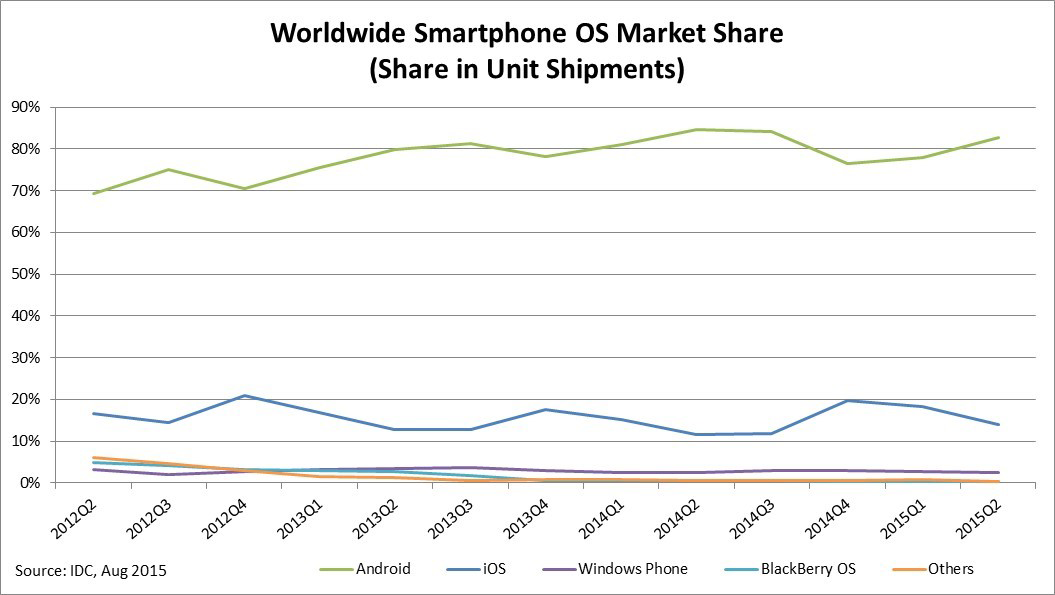
\includegraphics[scale=0.4]{img_03.png}
    \caption{Worldwide Smartphone OS Market Share} 
\end{center}
\end{figure}

2.	Which programming language and why?\\

-- Java for android application developing

Java is a general-purpose computer programming language that is concurrent, class-based, object-oriented, and specifically designed to have as few implementation dependencies as possible. As of now, Java is one of the most popular programming languages in use, particularly for client-server web applications, with a reported 9 million developers. Java was originally developed by James Gosling at Sun Microsystems (which has since been acquired by Oracle Corporation) and released in 1995 as a core component of Sun Microsystems' Java platform. The language derives much of its syntax from C and C++, but it has fewer low-level facilities than either of them. And Java is the best suitable language to develop the application in android OS.\\

-- C for IDE

We should do many tests to recognize various users' postures using pressure values getting from FSR-406 pressure sensors. So, we use the open-source Arduino Software (IDE) and the best proper language to use this program is C. The open-source Arduino Software (IDE) makes it easy to write code and upload it to the board. It runs on Windows, Mac OS X, and Linux. The environment is written in Java and based on Processing and other open-source software. This software can be used with any Arduino board.\\

-- PHP

PHP is a server-side scripting language designed for web development but also used as a general-purpose scripting language that is especially suited to web development. PHP is fast, flexible and pragmatic language. And PHP makes the user write dynamic web files because PHP follows many sentence forms used in C, Java, Perl etc. And there is excellent documentation we can refer to. http://www.php.net/ has really good documentation with helpful user-contributed gotchas and code snippets. We can also find tons of tutorials, etc. around the web.\\

3.	Provide a cost estimation for your built.\\

-- Cost for Server :

1 year for free. And after 1 year, there will be additional prices. We predict maybe about 1,000 people will use our service, and DAU (Daily Activity User) will be 300 around. So we will use t1. micro instance (AWS), and its prices are about 30 dollars per month: So may be there will be additional 360 dollars per year.\\

-- Cost for hardware

1)	Arduino

The Uno is a microcontroller board based on the ATmega328P. It has 14 digital input/output pins (of which 6 can be used as PWM outputs), 6 analog inputs, a 16 MHz quartz crystal, a USB connection, a power jack, an ICSP header and a reset button. It contains everything needed to support the microcontroller; simply connect it to a computer with a USB cable or power it with a AC-to-DC adapter or battery to get started. The Uno board and version 1.0 of Arduino Software (IDE) were the reference versions of Arduino, now evolved to newer releases. The Uno board is the first in a series of USB Arduino boards, and the reference model for the Arduino platform; for an extensive list of current, past or outdated boards see the Arduino index of boards.\\

2)	Pressure Sensors

The model 406 FSR is a single-zone Force Sensing Resistor optimized for use in human touch control of electronic devices such as automotive electronics, medical systems, and in industrial and robotics applications. FSRs are two-wire devices. They are robust polymer thick film (PTF) sensors that exhibit a decrease in resistance with increase in force applied to the surface of the sensor. It has a 39.6mm square active area and is available in 4 connection options. Interlink Electronics FSR 400 series is part of the single zone Force Sensing Resistor family.\\

3)	Bluetooth Module

HC-06 is a serial port module composed in SMD form which is possible to be replaced easily. It also uses the connection between the bluetooth Master module in either PC or mobile device and embedded system in substitution of the serial port. 

Arduino receives the input values, which the four pressure sensors perceive, through the breadboard and sends those values to the Android Application via bluetooth communication with the mobile phone. The system flow is shown in Figure 3.2.\\

\begin{figure}[htbp]
\begin{center}
    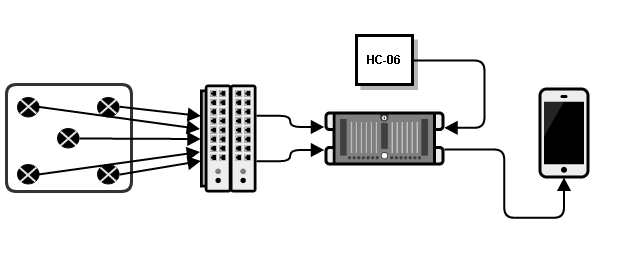
\includegraphics[scale=0.4]{img_01.png}
    \caption{System Flow} 
\end{center}
\end{figure}

Therefore, we need 4 pressure sensors, Arduino, bluetooth module, bread board, USB cable and jump wire MM. The specific products' cost is shown in Table 3.1.\\

%\begin{table}

\begin{tabular}{|c|c|c|c|}\hline


Products & Prices & Quantities & Costs \\ \hline \hline

Pressure Sensor & 14,000 & 4 & 56,000  \\

FSR-406 &  & & \\ \hline 

Arduino Uno R3 & 7,500 & 1 & 7,500 \\ \hline

Bluetooth Module & 6,000 & 1  & 6,000 \\

HC-06 & & &\\  \hline

Bread Board & 4,500 & 1 & 4,500 \\\hline

USB Cable & 500 & 1 & 500  \\ \hline

Jump Wire MM& 70 & 50 & 3500  \\ \hline

\multicolumn{3}{|c|}{Total} & \multicolumn{1}{|l|}{78,000} \\ \hline 

\end{tabular} \\\\

%\end{table}

4.	Provide clear information of your development environment. (e.g., version of software, OS version, your computer resources)\\

-	Android develop

1)	Windows : Windows 10

2)	Android Studio 1.5.1 / Android 4.4.4 Kitkat\\

-	Arduino develop 

3)	Windows : Windows 10

4)	Arduino 1.6.8 (IDE)\\


5.	Using any commercial cloud platform (e.g., Amazons EC2) is definitely a BONUS.\\

 We will use Apache Web Server because it is the world's most widely used web server software. As of June 2013, Apache was estimated to serve 54.2 percent of all active website and 53.3 percent of the top servers across all domains. (The most important reason is we have already apache web server.)\\

Apache Web Server has some features:

- easy and fast customizing using module.

- It can handle many traffic easily.

- It can control web server more delicately

- It is tested enough, so it is very stable.\\

\subsection{Software in use}

-	Footlogger

3L-Labs, internal venture corporation, developed a smart wearable device 'FootLogger'. It is insoles with some pressure sensors which analyze users' steps. This device can be used for health care, sports and entertainment.\\

Healthcare

- Monitors recovery after surgery

- Assesses balance of diabetics

- Allows for monitoring of prescribed exercises 

- Monitors safety and activity of senior citizens

- Activity tracking (calories, distance, time)

- Early prediction of dementia and spinal disease

- Early prediction of accidents from falling

- Monitors rehabilitation (stroke, paralysis)\\

Sports

- Can monitor distance traveled

- Monitors golf stance and gives coaching

- Marathon/jogging aid

- Out-toeing/in-toeing gait identification, provides 

gait coaching
 
- Kids' correct posture coaching

- Can be applied to every sport\\

Entertainment

-  Daily log (standing, sitting, walking)

-  Personality analysis

-  Daily mood analysis

-  Smartphone game input device\\

\begin{figure}[htbp]
\begin{center}
    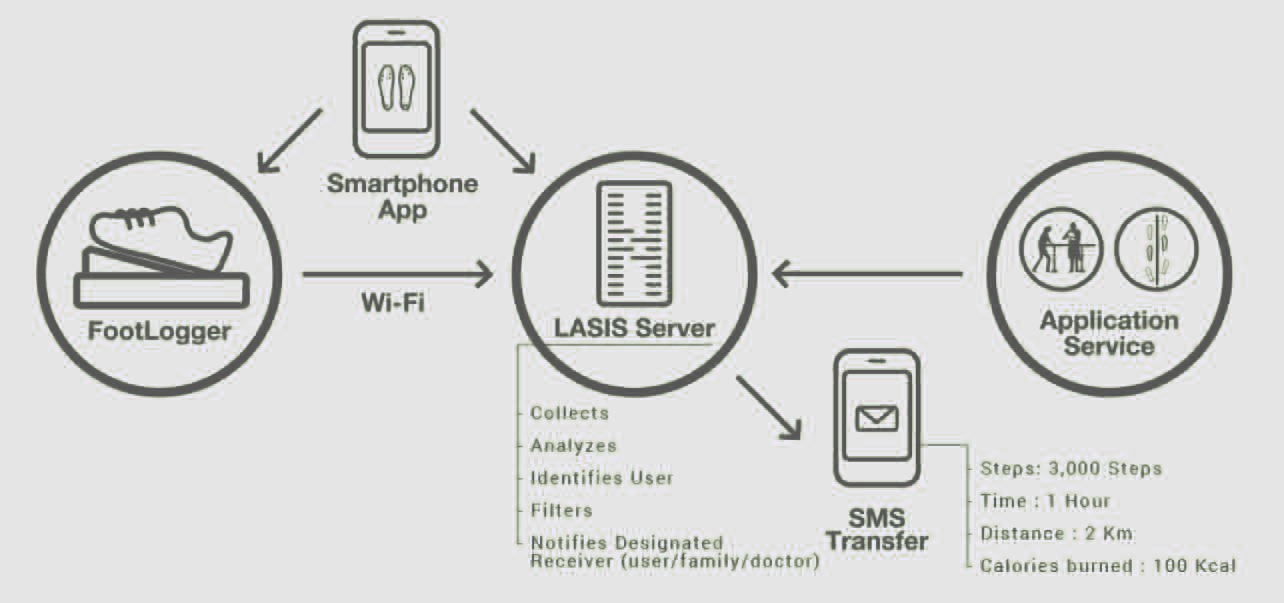
\includegraphics[scale=0.33]{img_05.jpg}
    \caption{Footlogger} 
\end{center}
\end{figure}

\subsection{Task distribution\\\\\\}

\renewcommand{\arrayrulewidth}{1pt}


%\begin{table}

\begin{tabular}{|c|c|l|}\hline
Role & Name & Task description and etc.\\ \hline \hline

&  &  -- Test the application in \\ 

&  &  various postures. \\

User & Minsoo & -- Require bugs to be fixed.  \\ 

& Choi & -- Demand the all of his data. \\ 

&  & -- Require additional functions. \\ \hline

&  &  -- Develop the application using\\ 

Software & Taejin & Arduino and pressure sensor. \\ 

Developer & Kim & -- Fix bugs. \\ 

&  & -- Develop additional functions\\ 

&  & according to users' needs. \\ \hline

&  &  -- Monitor the progress of the project. \\ 

Development & Hakjun & -- Make a overall plan about \\ 

Manager& Kim & developing program and managing \\ 

&  & the budget.\\

&  & -- Reflect users'needs \\ \hline

\end{tabular}

%\end{table}

\section{Specifications}

\subsection{Modeling for Specifications \\}


\begin{figure}[htbp]
\begin{center}
    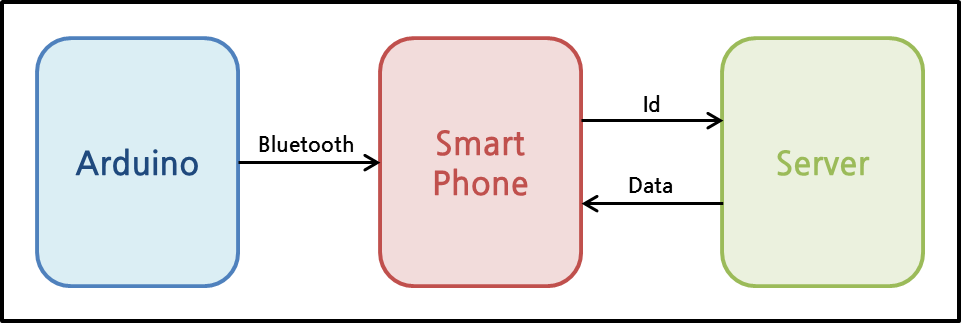
\includegraphics[scale=0.55]{img_04.png}
    \caption{Basic structure} 
\end{center}
\end{figure}


 Arduino receives some of the pressure value from the pressure sensor. And arduino sends the values to smart phone using HC-06. HC-06 is a Bluetooth Module. Then smart phone application determines posture of the user by analyzing the values. After that, smart phone calculates the time for holding the posture. The data of time will be sent to server, and saved at server.
At the same time, the application will receive the user's whole data from server. Then, the application will display the data by data visualization.\\\\

\subsection{Posture Recognition using pressure sensor}
 We made a kind of cushion for measuring pressure force. The dimensions of the chair and cushion are shown in Table 4.1. And we used FSR-406 pressure sensor model to get proper pressure value for recognizing person's changing posture. The dimensions of FSR-406 are shown in Figure 4.2\\
 
\emph{Table}

\begin{figure}[htbp]
\begin{center}
    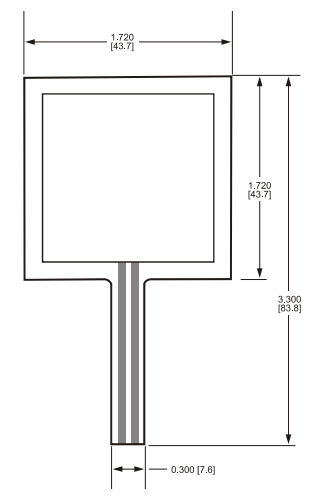
\includegraphics[scale=0.6]{img_06.png}
    \caption{Dimensions of FSR-406} 
\end{center}
\end{figure}

The reason why we choose the FSR-406 is the specifications of FSR-406 are suitable to make the posture recognition cushion. This sensor is very thin and hence can be easily bent to fit, so a user can sit down on the seat comfortably. Since the sensor sheet is light and thin, it can be carried anywhere and used in various situations in daily life. And the active area is appropriate to get pressure value when person changes his or her posture. FSR-406 specifications are shown in Table4.2.

\emph{Table}

FSRs are two-wire devices with a resistance that depends on applied force. For specific application needs please contact Interlink Electronics support team. An integration guide is also available. For a simple force-to-voltage conversion, the FSR device is tied to a measuring resistor in a voltage divider configuration. This is shown in Figure 4.3. The output is described by the equation:


\begin{displaymath}
\qquad\mathrm{V}_{out} =\frac{{R}_mV+}{({R}_M+{R}_{FSR})}
\end{displaymath}

In the shown configuration, the output voltage increases with increasing force. If ${R}_{FSR}$ and ${R}_{M}$ are swapped, the output swing will decrease with increasing force. These two output forms are mirror images about the line ${V}_{out}$  = $(V+) / 2$. The measuring resistor, ${R}_{M'}$ is chosen to maximize the desired force sensitivity range and to limit current. Depending on the impedance requirements of the measuring circuit, the voltage divider could be followed by an on-amp. A family of FORCE vs. ${V}_{out}$ curves is shown on the graph above for a standard FSR in a voltage divider configuration with various ${R}_{M}$ resistors. A $(V+)$ of $+5V$ was used for these examples.

\begin{figure}[htbp]
\begin{center}
    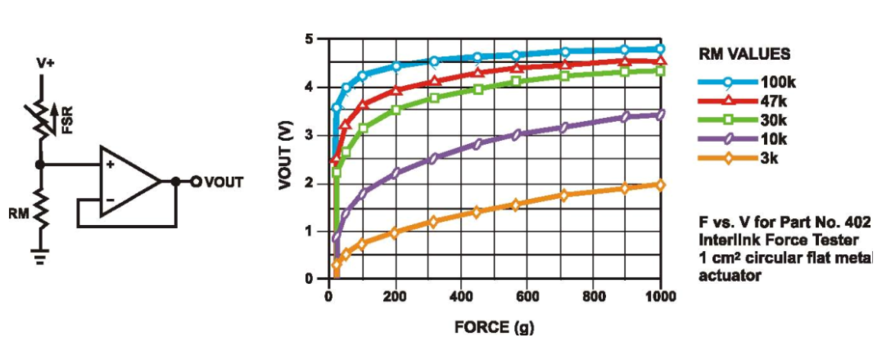
\includegraphics[scale=0.375]{img_07.png}
    \caption{Typical Schematic and force curve of FSR-406} 
\end{center}
\end{figure}

To recognize difference of sitting posture, we have to make the cushion with proper number of pressure sensors. So, we arranged five pressure sensors to the five points in the cushion. The five points are 'Left-front', 'Right-front', 'Center', 'Left-back', 'Right-back' and this classification is shown in Table 3. And the pressure values are transmitted to Arduino board through bread board. The pressure sensors' spot position is shown in Figure 4.4.

\emph{Table}

\begin{figure}[htbp]
\begin{center}
    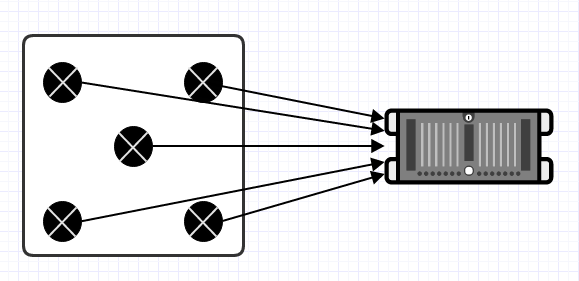
\includegraphics[scale=0.5]{img_08.png}
    \caption{Pressure sensors' spot position} 
\end{center}
\end{figure}

\subsection{Posture classification\\}

In this part, we describe a way of classifying sitting postures. Posture classification involves three basic issues. One issue is person dependency. Different persons would obviously sit in different ways. Even the same person might sit on different parts of the seating face. One ways to resolve this problem is to normalize pressure distributions by standardizing different postures when workers sit in the chair. The classification of seven postures is shown in Table 4.4.

\emph{table}

Second issue is the time depedency. We have to push alarm to users when they are doing wrong postures. So, it is needed to decide when we do alarm function. We set time standard from 1 minute to 10 minutes. User could select time when user gets push alarms while user keeps wrong posture. 
   And the last issue is weight dependency. The sensor values would increase linearly or non-linearly with an increase in weight. Therefore, it would be effective to divide the sensor values by the total value. And the each user's pressure value is different when user does 'Normal' posture. So, if user registers in our application, the user's initial pressure values are saved in the database and our algorithm uses each user's data to recognize posture. And we offer the function which initializes user's weight in the application. 

\subsection{Specification for front-end application pages\\}



 --	Log-In Page\\

\begin{figure}[h]
\begin{center}
    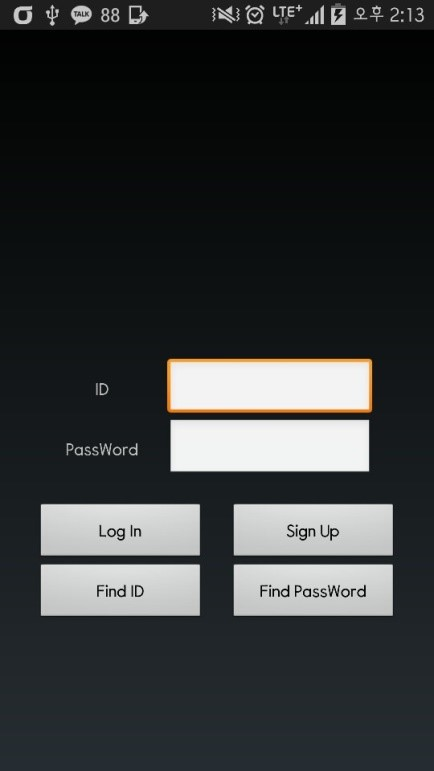
\includegraphics[scale=1]{img_10}
    \caption{Log-In Page} 
\end{center}
\end{figure}

 This page is the first page of the application. To import the posture data, you have to log in first. Your working posture records will be saved in your server with your ID. If you do not have an ID, you can click the Sing Up  button. Or, if you forgot your ID or password, you can find it using Find ID button or Find Password button. Once you log in, your ID and password will be automatically saved. Even when you log in via another phone, you can  open your records with ease since your posture records are imported from your ID only.\\

 -- Sign-Up Page\\
 
\begin{figure}[h]
\begin{center}
    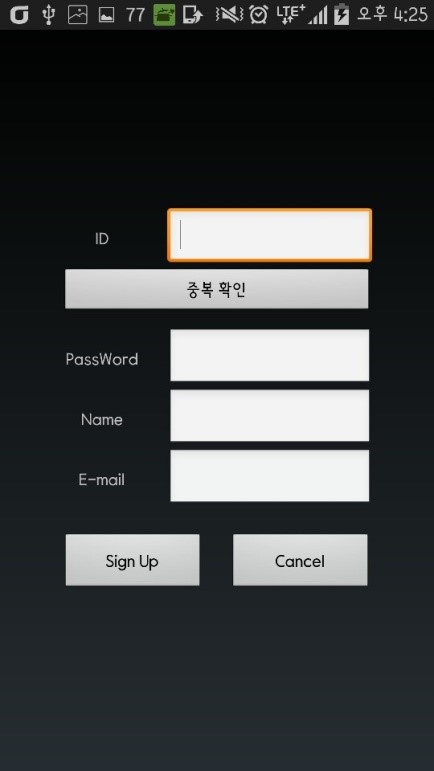
\includegraphics[scale=1]{img_11}
    \caption{Sign-Up Page} 
\end{center}
\end{figure}

 This page is where a user with no ID can create a new ID. Since ID will be the Primary Key of the User DB that will be saved in the server, it should not be overlapped. So, it is mandatory for you to double-check your ID. There is  no limit in the length of the password and the password will be replaced with other letters, such as ****, as soon as you enter your password for the sake of absolute confidentiality.

 Name and E-mail will be used for discerning between members and non-members. And, they will also be used for finding ID or Password in case you forgot it.\\

 -- Find ID Page\\

 Once you enter your E-mail that you entered during Sign-up process, it tells your ID on the screen.\\

 --Find Password Page\\

 Once you enter your E-mail that you entered during Sign-up process, it sends your password to your E-mail.\\
 
 --Now Page
 
\begin{figure}[h]
\begin{center}
    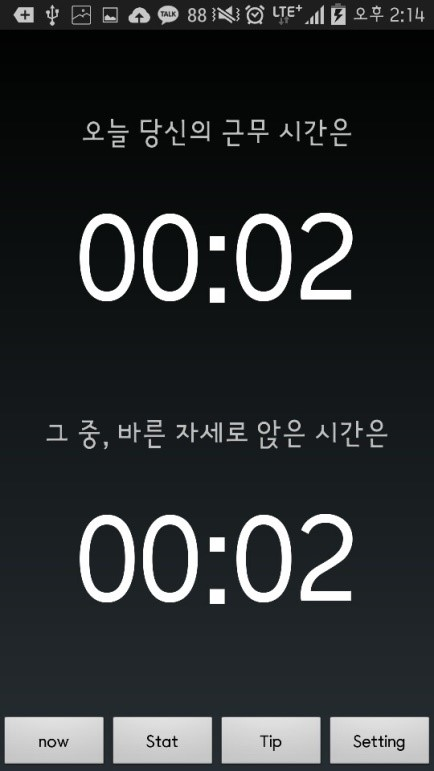
\includegraphics[scale=1]{img_12}
    \caption{Now Page} 
\end{center}
\end{figure}

 This page is the first page you see after you log in. There are 4 tabs in the tab bar below. 'Now' tab is the tab of the current page. If you click the 'Stat' tab, you can check your accumulated statistics on daily, weekly, monthly  and yearly basis. 'Tip' tab is where you can find images and videos of stretches or exercises useful for correcting posture. The last 'Setting' tab is for setting few functions related to this application.

 In this page, the app counts the number of hours you sit on the cushion that is composed of pressure sensor. This data will be exported on the screen in order for you to check your total working hour. (Upper Timer)
 
In specific, it counts the number of hours of your correct posture and bad posture separately. So, it is possible to check the number of hours of correct posture only. (Lower Timer)

 The number of hours exported from this page will be saved in the server as well. Moreover, once the user maintains a bad posture for a long time, the user will recieve a push notification that warns his/her long-time bad  posture.\\

 --Stat Page

\begin{figure}[h]
\begin{center}
    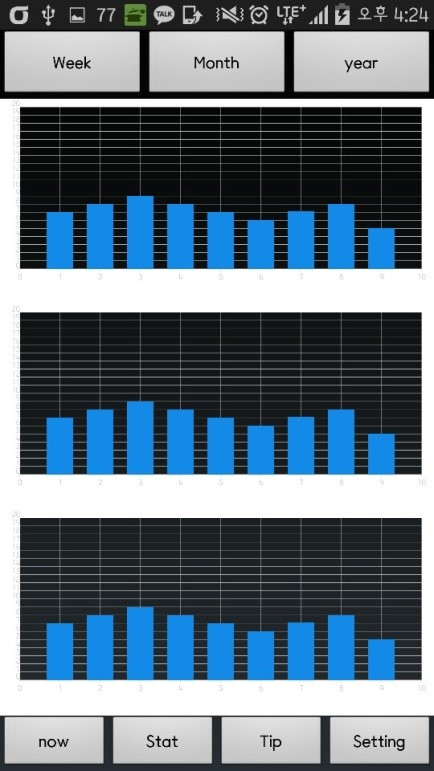
\includegraphics[scale=1]{img_13}
    \caption{Stat Page} 
\end{center}
\end{figure}

This page shows up as you click the Stat tab below. It is divided into 3 big graphs and has three tabs at the top of the screen. The graphs of this page are composed of individual time data saved in the server. Each of the  three graphs represents total working hour, the number of hours of correct posture and the bad posture.
The x-axis of this graph changes according to the upper tab of the screen. The x-axis consists of 7 days in the 'Weekly' tab, 30 days in the 'Monthly' tab and 12 months in the 'Yearly' tab.
The y-axis of every tab consists of numbers from 0 to 24, which refer to the number of hours.

 The first graph will be presented as a Bar Chart that shows working hour of the days of the week in the 'Weekly' tab, daily working hour in the 'Monthly' tab and monthly average working hour in the 'Yearly' tab.
With the same principle, the second graph shows the number of hours of correct posture for each tab whereas the third graph shows the number of hours of the bad posture.\\

 --Tip Page

\begin{figure}[h]
\begin{center}
    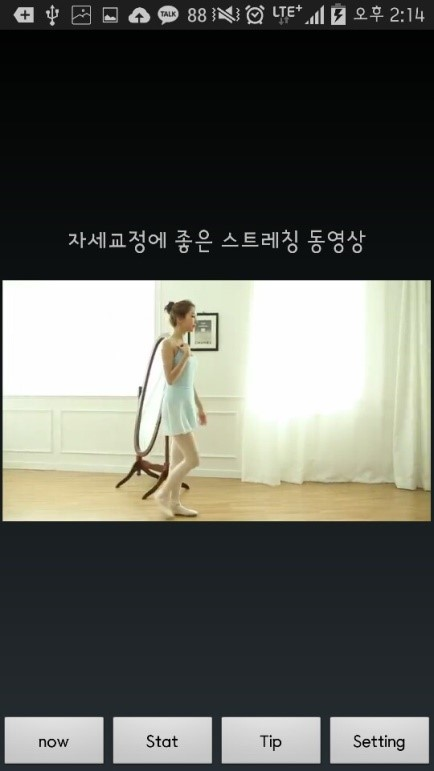
\includegraphics[scale=1]{img_14}
    \caption{Tip Page} 
\end{center}
\end{figure}

When clicking the Tip tab below this page, this page will show up. It exports images and videos of stretches or exercises useful for correcting posture as a customized ListView. The function of playing or pausing the video takes the similar format with Youtube. The first click plays the video and the second pauses it.\\

 --Setting Page

\begin{figure}[htbp]
\begin{center}
    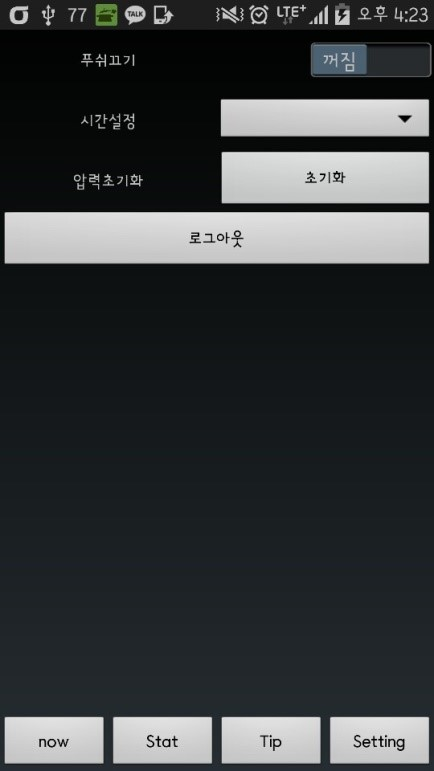
\includegraphics[scale=1]{img_15}
    \caption{Setting Page} 
\end{center}
\end{figure}

This page shows up when you click the 'Setting' tab below this page. The first function of this page, comprised of a ListView, is switching on or off the push notification. Essentially, if the user maintains a bad posture for a long time, the user will receive a push notification that warns his/her long-time bad posture. This function can be controlled by the user. 

The second function is to set the time when user gets push alarms while user keeps wrong posture. It ranges from minimum 1 minute to maximum 10 minutes. For example, if you set your time to 2 minutes and you maintain a bad posture for 2 minutes, you will directly receive a notification.

The third function resets the pressure value that matches the users' body. According to individuals' weight and environment, the pressure value differs. Hence, it is necessary to save individuals' initial pressure value of the  correct posture in the server. The last but not least function is log-out. It allows the user to log out from the app.\\\\\\\\\\\\\\\\\\\\





\subsection{Specifications for Server}

\quad 1) Filezilla \\
We use the [filezilla] to upload the data such like image, and text for exhibition. FileZilla is free-open source cross platform. It consists of filezilla client and filezilla server. It can used at windows, mac os, and linux. \\


\begin{figure}[htbp]
\begin{center}
%    \includegraphics[scale=0.2]{img_filezilla}
    \caption{filezilla01} 
\end{center}
\end{figure}


\begin{figure}[htbp]
\begin{center}
%    \includegraphics[scale=0.2]{img_filezilla02}
    \caption{filezilla02} 
\end{center}
\end{figure}

If artist want to upload the data of his exhibition, he needs to contact us and send the data to us first. After receiving data from artist, we can upload the exhibition data to our server. Then, data is stored at our web server, and wail the signal calling it.\\\\\\\\\\\\\\

\quad 2) Pgadmin \\

We use [pgadmin] for make and control the database. 
\begin{figure}[htbp]
\begin{center}
%    \includegraphics[scale=0.2]{img_pgadmin01}
    \caption{pgadmin} 
\end{center}
\end{figure}

In first picture, there are tables of our database. We made 5 tables.\\

\begin{figure}[htbp]
\begin{center}
%    \includegraphics[scale=0.2]{img_pgadmin02}
    \caption{pgadmin table01} 
\end{center}
\end{figure}

First, [bc.exh.device] table is for beacon id [PK](This beacon is at the entrance of the exhibition). At this table, we make the exhibition code and match to beacon id. And we make the exhibition code to.\\\\\\\\\\\\\\\\\\


\begin{figure}[htbp]
\begin{center}
%    \includegraphics[scale=0.2]{img_pgadmin002}
    \caption{pgadmin table02} 
\end{center}
\end{figure}

Second, [bc.exhibition] table is for  brief information about exhibition. Exhibition code is  [PK]. This table is connected to [bc.exh.device]table.\\

\begin{figure}[htbp]
\begin{center}
%    \includegraphics[scale=0.2]{img_pgadmin003}
    \caption{pgadmin table03} 
\end{center}
\end{figure}

[bc.file] table is for image files. There is the 3 type integers. Type integer 1 is for exhibition main image. It is used at My history page02, and Information page02. Type integer 2 is for thumbnail image of artwork. It is used at My history page 02. Type integer 3 is for the image of artwork. It is used My history page 03.\\\\\\\\\\\\\\


\begin{figure}[htbp]
\begin{center}
%    \includegraphics[scale=0.2]{img_pgadmin004}
    \caption{pgadmin table04} 
\end{center}
\end{figure}

[bc.pc.device] table is for beacon id[PK]. But this beacon is located nearby artwork. If user goes to artwork, then application recognize the beacon and send to server, this table. \\

\begin{figure}[htbp]
\begin{center}
%    \includegraphics[scale=0.2]{img_pgadmin005}
    \caption{pgadmin table05} 
\end{center}
\end{figure}

[bc.piece] table is for detail information about artwork. Artwork has its own code[PK]. \\\\\\\\\\\\\\\\\\\\

\section{Architecture Design and Implementation}
\subsection{Overall architecture}
\begin{figure}[htbp]
\begin{center}
%    \includegraphics[scale=0.5]{img_archi}
    \caption{Overall architecture} 
\end{center}
\end{figure}
\subsection{Directory organization}
\begin{figure}[htbp]
\begin{center}
%    \includegraphics[scale=0.5]{img_direc}
    \caption{Directory organization} 
\end{center}
\end{figure}
\quad
 \\\\\\\\\\\\\\\\\\\\\\\\\\\\\\\\\\\\\\\\\\\\\\\\\\\\\\\\\\\\\\\\\\\\\\\\\\\\\\\\\\\\\\\\\\\\\\\\\
\subsection{Code analysis}
\quad 1) Splash\\\\
-purpose : To show a cover page during the program is loading on the device. \\
\\ -functionality : Splash is a kind of loading screen. The function of splash is gaining time to get data which is necessary for program. Additionally, we can promote our application name during splash time.\\
\\ -location of source code : SmartBrochure/appsrc/java/com/example/jay/smart\_broch
ure/Splash.java\\
\\ -class components\\
\\ a. 'onCreate' method is implemented firstly in the activity class like main() method in JavaSE. In the onCreate, setContentView shows basic layout which is used to compose main page. By using postDelayed in handler, this method can do function how long loading page appear. \\
\\ b. onCreateOptionsMenu method does initializing option menu of activity.\\
\\c. In onOptionsItemSelected method, Handle action bar item clicks here. The action bar will automatically handle clicks on the Home/Up button, so long as you specify a parent activity in AndroidManifest.xml.\\
\\ -how/why you used it : If you want to implement some program, the program needs time to get source which is vital for program. Splash does function which gains time getting data.\\\\
\quad 2) SearchBle\\\\
-purpose : To search beacon which uses Bluetooth Low Energy(BLE). \\
\\ -functionality : SearchBLE is implemented on application background. Usually almost classes inherit Activity class, but SearchBLE inherits Service class because searching function isn’t seen in the smartphone screen but implemented background. This service searches the BLE devices around the user and check if the BLE address is in our database or not. If the address is in our database and it is not the one that user already visited, this service will send the BLE address to the server to get the information of the exhibition and give the push alarm to the user to get the brochure.\\
\\ -location of source code : SmartBrochure/appsrc/java/com/example/jay/smart\_broch
ure/SearchBle.java\\
\\ -class components\\
\\ a. BroadcastReceiver uses the onReceive() method to get the state of the Bluetooth. If the devices’ Bluetooth is on, this starts the Searching BLE service, by using Timer instance, which makes the period of searching time and so on. If the Bluetooth becomes off, this stops searching BLE devices by calling cancel() method in the Timer instance and scanLeDevice() method by giving the parameter as “false”. It is used to realize operation when application completed specific task.\\
\\ b. Timer is basic class in Android. By using Timer class, we can set schedule when searching starts and how long search beacon. When we use Timer instance, Android appreciate '1 = 1 millisecond'. Therefore, if we want to set searching time 3 seconds, we have to put value 3*1000. In our code, we set it as schedule(search, 10*1000, 20*1000); which meanse it will start searching after 10 secs, and for 20secs, and it will rotate.\\
\\ c. onLeScan's main function is using Handler, which means it will use the Threads. In the run() method, which is working on the thread, the application will check the database if there is a valid address that our service is using, and if two are matched, this will check whether the user has visited to this exhibition by searching the History table in the Database class. Only when there is no history about the beacon address, it will send the address and the code to the server to get the information about the exhibition and will give the device push-alarm which will help the user to get the brochure. When we search beacon, there are so many beacons even if we don't need. If we don’t figure out whether it is valid or not, we have to send all beacon data which are not necessary to server. That can provoke wasting of data use. By using this method, we can send appropriate beacon data to server. Additionally, if an appropriate beacon data sent to server, the method will save the address in the temporary ArrayList<String> variable to prevent sending same address to the server over and over again. If we don’t do this, push alarm will come continuously while audiences watch the exhibition.\\
\\ d. sendId() method is the core part of this service which sends the data to the server and get the data from server to the application. Using HashMap<String, Object> type of variable, we put the beacon id and make it to JSONObject, which server wants as the data type to get from the device. After that, by using DefaultHttpClient, the device will get the data from the server as JSONArray type, so we will cast the datatype that we want to use, and make the push alarm by using NotificationCompat class.\\
\\ -how/why you used it : By using  Auto\_Start class, we made SearchBLE service start when the devices’ booting is completed, only if the auto-search option is on. Therefore, if the user set up the option as on, the user doesn’t need to turn on the application to get the brochure. By only turning on the Bluetooth, this service will search the beacons around the user and send the data to the server and will notify the user by push alarm. This is one of the core concept of IoT..\\\\
\quad 3) MainActivity\\\\
-purpose : To show main page and constitute tab view which consist of My, Info, and Setting for customer.\\
\\ -functionality : MainActivity is the body of SmartBrochure. Most classes are used in this class. The main function is showing main page which is made up of several components.\\
\\ -location of source code : SmartBrochure/appsrc/java/com/example/jay/smart\_broch
ure/MainActivity.java\\
\\ -class components\\
\\ a. turnOnBT method instructs whether to turn on or turn off Bluetooth to customers by dialogue. If Bluetooth is turned on before starting application, notification dialogue will not occur on the device.\\
\\ b. getServiceTaskName checks if the SearchBLE service is now running or not. If it is not running, we will start SearchBLE service in order to search the beacons if the Bluetooth is on.\\
\\ c. We overrode onDestroy() method.  When the application destroys, we need to turn of the SearchBLE service too, if the auto-searching option is off. Therefore, we opened database in this method to check if the option is turn on or off.\\
\\ -how/why you used it : MainActivity is foundation of application. We build the tab activity to make the tabs for the pages, My, Info, Setting. We made this class inherit TabActivity, but we will fix this to FragmentActivity because TabActivity is deprecated.\\\\
\quad 4) My\\\\
-purpose : My\_Clicked shows the list of art work. The list includes name and image of each art work.\\
\\ -functionality : First tab button on the main page and if you execute SmartBrochure, you can see my page firstly. If you click one of the list, list of the exhibition work appears.\\
\\ -location of source code : SmartBrochure/appsrc/java/com/example/jay/smart\_broch
ure/My.java\\
\\ -class components\\
\\ a. sendId method does the same function as the sendId method in the SearchBLE. We get the exhibition code and the BLE address that is already saved in the Database when the user visitied the exhibition, and send them to the server to get the exhibition brochure from the server. After server gets the beacon data and the valid exhibition code, the servier will send the exhibition data (exhibition name, list of work, image and so on) to SmartBrochure and we go to the My\_Clicked class to show the brochure.\\
\\ b. customAdapter's main function is giving data to list view. In the customAdapter, getView method put the data to the list.\\
\\ c. We made this listview get the OnItemClickListner, so when user touch the list, the page will go to the My\_Clicked page which gets the data of the exhibition.\\
\\ -how/why you used it : My page gets the list of history from the Database and put them to the listview. We thought that listview is the best way to show the list to the user. Between My and My\_Clicked, the data communication between the device and server occurs.\\\\
\quad 5) My\_Clicked\\\\
-purpose : My\_Clicked shows the list of art work of the exhibition that the user visited before. Most of the function is as same as Push\_Clicked.\\
\\ -functionality : My\_Clicked class must need to communicate with server in order to get the brochure from the server. In the My page we sent the id and exhibition code to the server, we will get the brochure data from the server in My\_Clicked page and will show the brochure.\\
\\ -location of source code : SmartBrochure/appsrc/java/com/example/jay/smart\_broch
ure/My\_Clicked.java\\
\\ -class components\\
\\ a. ImageLoaderConfigurationbition is used to show the image from the image URL we get from the server. In the application, image file is not anywhere. However, in order to use work image, we can use server. When we need some image file, we get URL which has image from server. In other words, just borrow image file when we need. If we go out of the page which has image, image file is removed from application.\\
\\ b. We use customAdapter and OnClickListener, and so on, which is used in other pages also.\\
\\ -how/why you used it : We communicate with the server here again, because we don’t want to save so many imagefiles to the application database, which will cause some problems of the storage of the device. Instead, we chose to communicate with the sever again, so we gets all of the data we use here from the server.\\\\
\quad 6) Push\_Clicked\\\\
-purpose : Push\_Clicked also shows the list of art work. The list includes name and image of each art work.\\
\\ -functionality : Push\_Clicked class must need to communicate with server in order to get the brochure from the server. In the Push page we sent the to the server, we will get the exhibition code and brochure data from the server in Push\_Clicked page and will show the brochure when user clicked the push alarm button which was sent before.\\
\\ -location of source code : SmartBrochure/appsrc/java/com/example/jay/smart\_broch
ure/Push\_Clicked.java\\
\\ -class components\\
\\ a. ImageLoaderConfigurationbition is used to show the image from the image URL we get from the server. In the application, image file is not anywhere. However, in order to use work image, we can use server. When we need some image file, we get URL which has image from server. The image URL or the Image file that we used here will never be stored in the database.\\
\\ b. In the onCreate method, we get the data of the brochure. Here, we need to save the beacon’s id and exhibition code in the database in order to keep the history of user’s exhibiting. We used History class to save the exhibition title, name, and the BLE address. After that, we use the addHistory method to save it in the database with SQLite.\\
\\ -how/why you used it : Push\_Clicked is very similar with My\_Clicked. However, they are different in sending id value to server. My\_Clicked is focused on existing exhibition information. In contrast, Push\_Clicked is focused on new information from beacon search. While My\_Clicked page sent the beacon’s id and exhibition code, in Push\_Clicked page, we send only the beacon’s id that SearchBLE service has searched to the server. \\\\
\quad 7) Explanation\\\\
-purpose : Explanation class has function which gives the detailed description about art work. Users can read the detailed image and the explanation of the specific work that the user wants to see the detail.\\
\\ -functionality : When you click one of the art works in the list(in the My\_clicked or Push\_Clicked), Explanation class is implemented. In this process, communication with server is very essential like My\_clicked or Push\_Clicked. Explanation also use image by using URL from server.\\
\\ -location of source code : SmartBrochure/appsrc/java/com/example/jay/smart\_broch
ure/Explanation.java\\
\\ -class components\\
\\ a. In the Explanation class, onCreate method's main function is setting ImageView and TextView which will be used after getting data from the server. They are given from server. At the end of this method, we call the setExplanation() method to set the data.\\
\\ b. setExplanation method uses some function like DisplayImageOptions and ImageLoaderConfiguration. By using them, we set the image from the imageURL, and the explanation of the artwork.\\
\\ -how/why you used it : Explanation class is the most informative section in our application. Like My\_Clicked, we use server to use adequate image, because image data is very important in exhibition information. \\\\
\quad 8) Info\\\\
-purpose : Info notifies several exhibitions’ information which is what is exhibiting now.\\
\\ -functionality : Second tab button on the main page so if you execute SmartBrochure, you can't see Info page firstly. If you click Info button, list of several exhibition which are exhibition now appears. We get this information from the server, which means, if the user click on the Info tab button, the device will communicate with the server to get the information.\\
\\ -location of source code : SmartBrochure/appsrc/java/com/example/jay/smart\_broch
ure/Info.java\\
\\ -class components\\
\\ a. In the Info class, sendId method is the important method because uses server like several other classes. Here, the device will just send the url Id and then the server will send the list of the exhibitions only.\\
\\ b. Here, we also used ListView to show the list of the exhibitions which users can go to and get the brochure and see the artworks now.\\
\\ -how/why you used it : This is just a basic page of ListView, to show the list of exhibitions our service is providing. We will get the list from the server when user tries to go to the info page. If the Internet is not on on the device, this page will show nothing beacause it will not get any data from the server. The reason why we made this page is that we thought that users might need the information of the exhibitions and can choose the exhibition that they want to go. They will choose one or several of the exhibitions from the list and when they go to the exhibitions, they can get the brochure on their device.\\\\
\quad 9) Info\_Clicked\\\\
-purpose : Info\_Clicked shows exhibition name, location, date and brief explanation.\\
\\ -functionality : Info\_Clicked class also must need communication with server. If application sends the id value which is in the database, after that server sends information about the exhibition which is correct with id to application.\\
\\ -location of source code : SmartBrochure/appsrc/java/com/example/jay/smart\_broch
ure/Info\_Clicked.java\\
\\ -class components\\
\\ a. In setInformation, there are so many function to make Info\_Clicked class. To show title, explanation, date and address, use text view.  ImageLoaderConfigurationbition is also used for implanting image like My\_Clicked. In the application, image file doesn't store anywhere. However, in order to use work image, we can use server. When we need some image file, we get URL which has image from server. In other words, just borrow image file when we need. If we go out of the page which has image, image file is removed from application.\\
\\ -how/why you used it : Info\_Clicked knows us information about exhibition that we can go. People who are interested in art want to kwon exhibition information which they can go nowadays. Also we add some data like exhibition image, brief explanation and so on. These information will satisfy user's needs.\\\\
\quad 10) Setting\\\\
-purpose : Setting is used to set automatic search by using Bluetooth and show the version of the application.\\
\\ -functionality : By setting, users can choose whether searching the beacon devices automatically or not. If you want to get exhibition data when you hang around outside, ust set 'automatic search' on in the setting.\\
\\ -location of source code : SmartBrochure/appsrc/java/com/example/jay/smart\_broch
ure/Setting.java\\
\\ -class components\\
\\ a. In the onCreate method, auto\_search find signal from beacon which is around user. btn\_onoff set that user turn on/off the automatic search function. At first, we get the on/off data from the database to show the user the current setting.\\
\\ b. In the onCreate method, auto\_search find signal from beacon which is around user. btn\_onoff set that user turn on/off the automatic search function. At first, we get the on/off data from the database to show the user the current setting.\\
\\ -how/why you used it : If user always turn on Bluetooth and turn on auto\_search function, user's smartphone battery will be consumed rapidly. Therefore, we thought it is very important to set these functions on/off. This function can save users’ smartphone battery and satisfy the users’ preference.\\\\
\quad 11) Database\\\\
-purpose : To store the lists of beacons that our service is using/ will use, the history of the user’s own exhibitions that he/she has visited and got the brochure from it, and save the setting of automatic beacon searching preference.\\
\\ -functionality : In the services and pages of our service, especially SearchBLE, My, and Setting, we need to use the database to keep the user’s preferences and the history of visiting the exhibitions.\\
\\ -location of source code : SmartBrochure/appsrc/java/com/example/jay/smart\_broch
ure/Database.java\\
\\ -class components\\
\\ a. First, the database class inherits SQLiteOpenHelper to use the database with SQLite.\\
\\ b. setExplanation method uses some function like DisplayImageOptions and ImageLoaderConfiguration. By using them, we set the image from the imageURL, and the explanation of the artwork.\\
\\ c. init() method - when the user first downloaded this application, the device doesn’t have any database, but we need the list of the beacons that we use. Therefore, when the application was on for the first time, call init() method in Database.java and this will make the list of the beacons and set the ONOFF preference “0”, which means “off”, as default.\\
\\ d. getOnoff() method - search the CheckOnOff table and get ONOFF row and return in order to check if the onoff setting is on or off.\\
\\ e. editOnoff() method - get String value as the parameter and edit the ONOFF row in the CheckOnOff table. \\
\\ f. getList() method - return the list of the S-Brochure table.\\
\\ g. updateBeacons() method - using Cursor class and ContentValues class, update the beacons that out service use.\\
\\ h. getBeaconse() method - return the list of the beacons that we are using, to identify the BLE address that is valid for this application.\\
\\ i. addHistory() method - using the History class, add the beacon’s address and the name and code of the exhibition that user visited to the S\_Brochure table.\\
\\ j. getHistoryName(), getHistoryAddress(), and getHistoryCode() methods - three of these methods searches the DB and return the beacon’s address and the name and code of the exhibition that user visited with ArrayList<String> type.\\
\\ k. searchHistory() method - with the parameter of String type, search the DB to find if there is the same address in the DB.\\
\\ -how/why you used it : We developed this database with SQLite. If some classes(activities) needs the database information, they can instantiate the Database class and use the methods that we have made so that they will be able to access to the Database and get the information they need and edit the database if it is needed. The database is essential to our Smart Brochure service, since we need to manage the history of the user’s visiting exhibitions; if they want to read the previous brochure, they don’t need to go to the exhibition again if they have already visited. Also, the application needs to have the list of the beacons that it should search and send the information to the server, because there are a lot of BLE devices around us. Therefore, we had to give the application the list of beacons that it should send the information if one of them is sensed. Lastly, we have the function of auto-searching setting, so the database has the setting and can figure if the setting is on or off.\\\\
\quad 12) History\\\\
-purpose : To make it easier and flexible to keep the database.\\
\\ -functionality : There are several methods to get the data and give the date to the caller. Other classes will instantiate this class and save data in the object, and will send this object to the database.\\
\\ -location of source code : SmartBrochure/appsrc/java/com/example/jay/smart\_broch
ure/History.java\\
\\ -class components\\
\\ a. This class has getAddress(), setAddress(), getName(), setName(), getCode(), setCode() method to make the flexibility higher.\\
\\ -how/why you used it : We just made some methods to get and set the data to and from the database. We will use this class by making it instance in other classes. Save the data in the instance and transfer the instance to the Database. Without this method, it becomes more complex to keep the database.\\\\.\\\\\\\\\\\\\\\\\\\\\\\\\\\\\\\\\\\\\\\\\\\\\\\\\\\\\\\\\\\\\\\\\\\\\\\\\\\\\\\\\\\\\\\\\\\\\\\\\\\\\\\\\\\\\\\\\\\\\\\\\\\\\\\\\\\\\\\\\\\\\\\\\\\\\\\\\\\\\\\\\\\\\\\\\\\\\\\\\\\\\\

\section{Use Cases}

\begin{figure}[htbp]
\begin{center}
%    \includegraphics[scale=0.75]{img_flowchart}
    \caption{Application Flowchart} 
\end{center}
\end{figure}



.\\\\\\\\\\\\\\\\\\\\\\\\\\\\\\\\\\\\\\\\\\\\\\\\\\\\\\\\\\\\\\\\\\\\\\\\\\\\\\\\\\\\\\\\\\\\\\\\\\\\\\\\\\\\\\\\\\\\\\\\\\\\\\\\\\

\begin{figure}[htbp]
\begin{center}
%    \includegraphics[scale=0.5]{img_serverFlowchart}
    \caption{Server Flowchart} 
\end{center}
\end{figure}

.\\\\\\\\\\\\\\\\\\\\\\\\\\\\\\\\\\\\\\\\\\\\\\\\\\\\\\\\\\\\\\\\\\\\\\\\\\\\\\\\\\\\\\\\\\\\\\\\\\\\\\\\\\\\\\\\\\\\\\\\\\\\\\\\\\
\quad6-1) BLE searching and push notice
\begin{figure}[htbp]
\begin{center}
%    \includegraphics[scale=0.2]{img_capture01}
    \caption{BLE searching and push notice} 
\end{center}
\end{figure}\\
\quad If User turn on the bluetooth module, smartphone finds the BLE signal, and then Server sends to notice that information data about Exhibition is downloaded. If user touch the push notice, then temporary activity is open.\\\\\\\\\\\

\quad6-2) Temporary Activity01 \\
\begin{figure}[htbp]
\begin{center}
%    \includegraphics[scale=0.2]{img_capture02}
    \caption{Temporary Activity 01} 
\end{center}
\end{figure}\\
\quad This is the page when temporary page is open. It shows the information received from server. Upper-side of the page, there are the name and main image of exhibition. Under, there are the artwork lists which are displayed at the exhibition now user is seeing.\\\\\\\\\\\\\\

\quad6-2) Temporary Activity02 \\
\quad If the user touch one artwork, he can watch the detail of artwork. Of course every data is received from server. There are image, name, and detail descriptions of the artwork. 
\begin{figure}[htbp]
\begin{center}
%    \includegraphics[scale=0.18]{img_capture03}
    \caption{Temporary Activity02} 
\end{center}
\end{figure}
\\

\quad6-3) Main Application - My History Page01\\
\begin{figure}[htbp]
\begin{center}
%    \includegraphics[scale=0.2]{img_capture04}
    \caption{My History01} 
\end{center}
\end{figure}\\
\quad User will see this page when he run the application. It is the first page of main application. First, there is tab menu under the screen. By this tab menu, user can move to page he want to see.  This page is for user own. The data which he received from server and saw through temporary activity is stacked at this page. But this page only store the name of exhibition. Because the memory of smartphone. If user touch some exhibition which want to see again, then application send to the server the [eh.code] and get the data of that exhibition.\\\\\\\\\\\\\\\

\quad6-3) Main Application - My History Page02\\
\begin{figure}[htbp]
\begin{center}
%    \includegraphics[scale=0.2]{img_capture05}
    \caption{My History02} 
\end{center}
\end{figure}\\
\quad This page shows the detail information about the exhibition. User can see the brief details about the exhibition theme, the Artist, and the list of artwork which is displayed on that exhibition. \\\\

\quad6-3) Main Application - My History Page03\\
\begin{figure}[htbp]
\begin{center}
%    \includegraphics[scale=0.2]{img_capture06}
    \caption{My History03} 
\end{center}
\end{figure}\\
\quad If user touch any artwork at the My History Page01, user can see the detail information about that artwork like this page.\\\\\\\\

\quad6-3) Main Application - Information Page01
\begin{figure}[htbp]
\begin{center}
%    \includegraphics[scale=0.2]{img_capture07}
    \caption{Information Page01} 
\end{center}
\end{figure}

This is the second menu page of the application. User can move to this page from the other using tab menu under the screen. This page is for inform about the other exhibition. On the screen, there will be the list of exhibition that user has not seen yet. If user touch the INFO menu from other page, or swipe down the list, then application connect to the server([bc.exhibition]) and get the data of the list of the exhibition. It means, user can refresh the list whenever he wants.\\\\\\\\\\\\\\\\

\quad6-3) Main Application - Information Page02
\begin{figure}[htbp]
\begin{center}
%    \includegraphics[scale=0.2]{img_capture08}
    \caption{Information Page02} 
\end{center}
\end{figure}

If user select one exhibition, he can see the detail information about that exhibition such like the main image of the exhibition, information about the artist, the address of the exhibition and so on. \\\\\\\\\\\\\\\\\\\\\\\\\\\\\\\\\\\\\\\\\\

\quad6-3) Main Application - Setting Page
\begin{figure}[htbp]
\begin{center}
%    \includegraphics[scale=0.2]{img_capture09}
    \caption{Setting Page01} 
\end{center}
\end{figure}

User can turn on or off the function searching the BLE. - Turn on\\\\\\\\\\\\\\\\\\\\\\\\\\\\\\\\\\\\\\\\\\\\\\\\

\begin{figure}[htbp]
\begin{center}
%    \includegraphics[scale=0.2]{img_capture10}
    \caption{Setting Page02} 
\end{center}
\end{figure}

User can turn on or off the function searching the BLE. - Turn off\\\\\\\\\\\\\\\\\\\\\\\\\\\\\\\\\\\\\\\\\\\\\\\


\section{Software Installation Guide\\}
\quad8.1 How to install?

\begin{figure}[htbp]
\begin{center}
%    \includegraphics[scale=0.18]{img_install01}
    \caption{Searching at playsotre} 
\end{center}
\end{figure}

First, you have to access the playstore(android) or App Store(iOS) and search [SMART BROCHURE]. \\

\begin{figure}[htbp]
\begin{center}
%    \includegraphics[scale=0.18]{img_install02}
    \caption{Access the application page} 
\end{center}
\end{figure}

Second, click the [installation] button and download the [SMART BROCHURE] to your smartphone.\\

\begin{figure}[htbp]
\begin{center}
%    \includegraphics[scale=0.18]{img_install03}
    \caption{Downloaded to your smartphone} 
\end{center}
\end{figure}

Finally, you finish the installation. \\\\\\

\begin{figure}[htbp]
\begin{center}
%    \includegraphics[scale=0.4]{img_qrcode}
    \caption{install using QRcode} 
\end{center}
\end{figure}

Or, take this QR-code and access to the Playstore.\\\\\\\\\\\\\\\\

\section{Discussion}
\quad First of all, it was really hard for us to make the device communicate with beacons. Since we didn?t have any SDK that works with our beacons, we had to develop the code from nothing. Therefore, we searched about it on the website, which gives developers android APIs that it supports. In the Bluetooth category, we were able to find the information about Bluetooth Low Energy(BLE), which was necessary for our project. We had to study about the threads in the android, how to use Bluetooth in our application, and make it possible to run the service on the background of the device. In addition, we tried the communication of mobile application and the server for the first time. There were just a few of problem in the language, but we had to study about the JSON type, which we used to send and receive the information about the exhibitions and brochures. Moreover, we had a good chance to use the new programs, ?filezilla? and  ?pgadmin? we used for our server. Also, we had some trouble to use Latex and Github. We were very confused when professor told us that we have to use them. After a lot of tries, we were able to be used to use them. After getting used to it, we sincerely felt that it is really important to communicate with teammates in the project. From this class, we could deal with so many unfamiliar softwares and hardwares and learn how to go through the project from these process. Because there were a lot of our first tries, such as developing back-end server and linking it with the front-end applications. We also learned that keeping the deadline for each process is one of the most important components, in order not to delay the whole project. It was really a good experience for us and we feel that our ability and confidence has been improved a lot, so we would like to say thank you, professor. Additionally, (which you may already know about) we think it is better that doing usecase at the first step of the documentation because it would be better for us to draw the blueprint of our project documentation.
% An example of a floating figure using the graphicx package.
% Note that \label must occur AFTER (or within) \caption.
% For figures, \caption should occur after the \includegraphics.
% Note that IEEEtran v1.7 and later has special internal code that
% is designed to preserve the operation of \label within \caption
% even when the captionsoff option is in effect. However, because
% of issues like this, it may be the safest practice to put all your
% \label just after \caption rather than within \caption{}.
%
% Reminder: the "draftcls" or "draftclsnofoot", not "draft", class
% option should be used if it is desired that the figures are to be
% displayed while in draft mode.
%
%\begin{figure}[!t]
%\centering
%\includegraphics[width=2.5in]{myfigure}
% where an .eps filename suffix will be assumed under latex, 
% and a .pdf suffix will be assumed for pdflatex; or what has been declared
% via \DeclareGraphicsExtensions.
%\caption{Simulation Results}
%\label{fig_sim}
%\end{figure}

% Note that IEEE typically puts floats only at the top, even when this
% results in a large percentage of a column being occupied by floats.


% An example of a double column floating figure using two subfigures.
% (The subfig.sty package must be loaded for this to work.)
% The subfigure \label commands are set within each subfloat command, the
% \label for the overall figure must come after \caption.
% \hfil must be used as a separator to get equal spacing.
% The subfigure.sty package works much the same way, except \subfigure is
% used instead of \subfloat.
%
%\begin{figure*}[!t]
%\centerline{\subfloat[Case I]\includegraphics[width=2.5in]{subfigcase1}%
%\label{fig_first_case}}
%\hfil
%\subfloat[Case II]{\includegraphics[width=2.5in]{subfigcase2}%
%\label{fig_second_case}}}
%\caption{Simulation results}
%\label{fig_sim}
%\end{figure*}
%
% Note that often IEEE papers with subfigures do not employ subfigure
% captions (using the optional argument to \subfloat), but instead will
% reference/describe all of them (a), (b), etc., within the main caption.


% An example of a floating table. Note that, for IEEE style tables, the 
% \caption command should come BEFORE the table. Table text will default to
% \footnotesize as IEEE normally uses this smaller font for tables.
% The \label must come after \caption as always.
%
%\begin{table}[!t]
%% increase table row spacing, adjust to taste
%\renewcommand{\arraystretch}{1.3}
% if using array.sty, it might be a good idea to tweak the value of
% \extrarowheight as needed to properly center the text within the cells
%\caption{An Example of a Table}
%\label{table_example}
%\centering
%% Some packages, such as MDW tools, offer better commands for making tables
%% than the plain LaTeX2e tabular which is used here.
%\begin{tabular}{|c||c|}
%\hline
%One & Two\\
%\hline
%Three & Four\\
%\hline
%\end{tabular}
%\end{table}


% Note that IEEE does not put floats in the very first column - or typically
% anywhere on the first page for that matter. Also, in-text middle ("here")
% positioning is not used. Most IEEE journals/conferences use top floats
% exclusively. Note that, LaTeX2e, unlike IEEE journals/conferences, places
% footnotes above bottom floats. This can be corrected via the \fnbelowfloat
% command of the stfloats package.





% conference papers do not normally have an appendix


% use section* for acknowledgem



% trigger a \newpage just before the given reference
% number - used to balance the columns on the last page
% adjust value as needed - may need to be readjusted if
% the document is modified later
%\IEEEtriggeratref{8}
% The "triggered" command can be changed if desired:
%\IEEEtriggercmd{\enlargethispage{-5in}}

% references section

% can use a bibliography generated by BibTeX as a .bbl file
% BibTeX documentation can be easily obtained at:
% http://www.ctan.org/tex-archive/biblio/bibtex/contrib/doc/
% The IEEEtran BibTeX style support page is at:
% http://www.michaelshell.org/tex/ieeetran/bibtex/
%\bibliographystyle{IEEEtran}
% argument is your BibTeX string definitions and bibliography database(s)
%\bibliography{IEEEabrv,../bib/paper}
%
% <OR> manually copy in the resultant .bbl file
% set second argument of \begin to the number of references
% (used to reserve space for the reference number labels box)




% that's all folks
\end{document}
